\section{Related Work}
\label{sec:Related_Work}

As far as we know there is currently no other project aiming to better integrate git into Cloud9.
There are, however, several offline IDEs and stand-alone tools we took as inspiration for our
Cloud9 plugin \emph{gitc}.
Two of them we personally use are:
\begin{itemize}
	\item IntelliJ IDEA~\needcite
	\item gitx~\needcite
\end{itemize}
In the following sections we will show which features from those tools we intended to integrate into Cloud9.

\subsection{IntelliJ IDEA}
\label{subsec:IntelliJ_IDEA}

IntelliJ IDEA is a very rich Java IDE with plugins for various other languages such as Ruby, PHP and Scala.
The one git feature we set out to integrate into Cloud9 is the live diff inside the code editor.
This means that while you type the IDE shows you what changed and how as compared to the git index.

\begin{figure}
	\centering
	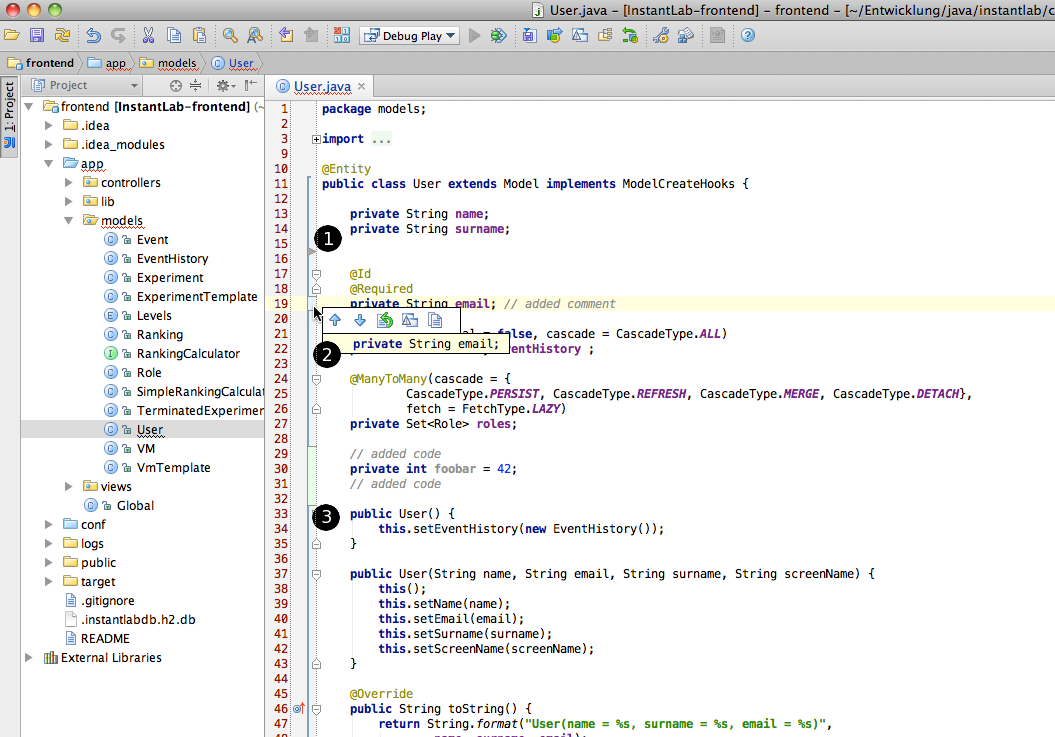
\includegraphics[width=0.9\textwidth]{images/idea-git.png}
	\caption{IntelliJ IDEA git integration}
	\label{fig:idea}
\end{figure}

In Figure ~\ref{fig:idea} you can see a screenshot of IntelliJ IDEA's code editor including the live diff.
At \circnum{1} there is a little gray triangle which marks deleted code.
You can see the deleted code by clicking on it.
Changed lines are marked via a blue strip on the editor's gutter (\circnum{2}).
By clicking that strip the original code is displayed.
Finally, as seen at \circnum{3}, added code is marked by a green strip.

\subsection{gitx}
\label{subsec:gitx}

Bundled with git comes a graphic tool called \emph{gitk} with which you can review local changes
and the history of your git repository. There are several similar tools that offer additional features.
One of those tools is \emph{gitx} for MacOS and one of the additional features is the ability to partially apply and revert
changes, while usually IDEs such as IntelliJ IDEA only allow you to commit files as a whole.

\begin{figure}
	\centering
	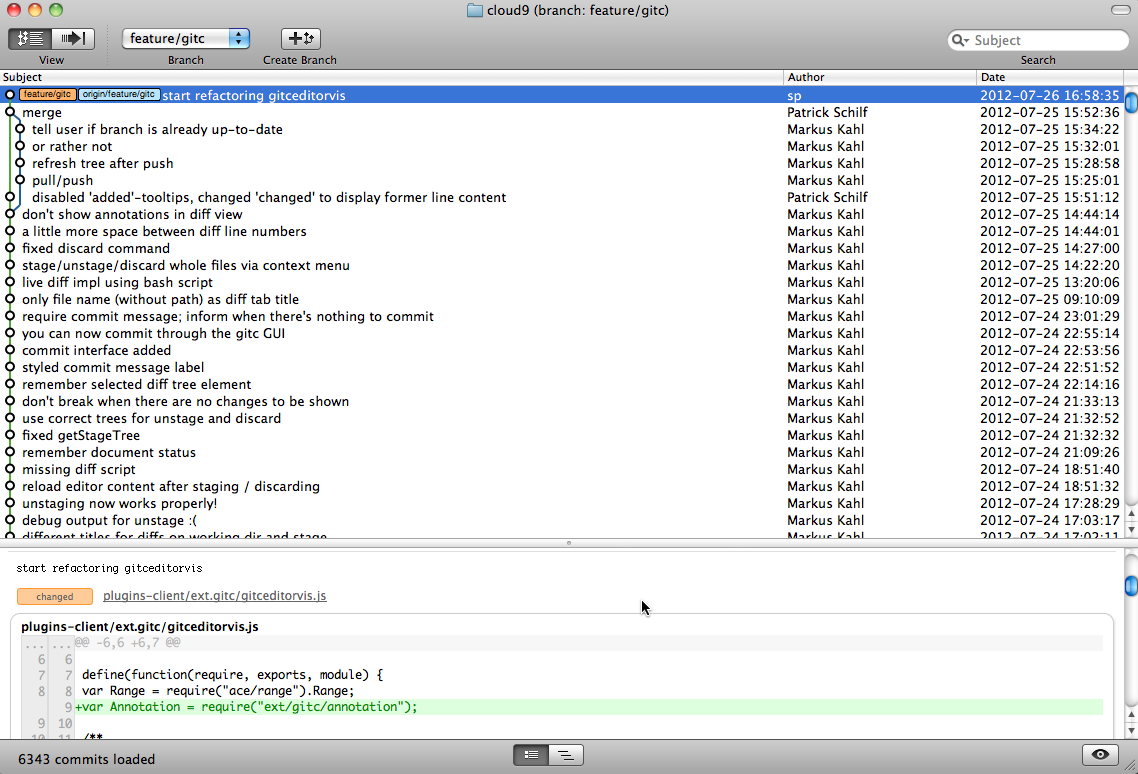
\includegraphics[width=0.9\textwidth]{images/gitx-history.png}
	\caption{gitx history view}
	\label{fig:gitx-history}
\end{figure}

Figure ~\ref{fig:gitx-history} shows gitx's history view where you can see the list of all commits.
Below the list of commits the diff for the selected commit is displayed.
Currently Cloud9 only provides a history of local changes independently from git. Another feature \emph{gitc} is supposed to add
is this git history view. Although it hasn't been implemented, yet.
\vspace{11 pt}

\begin{figure}
	\centering
	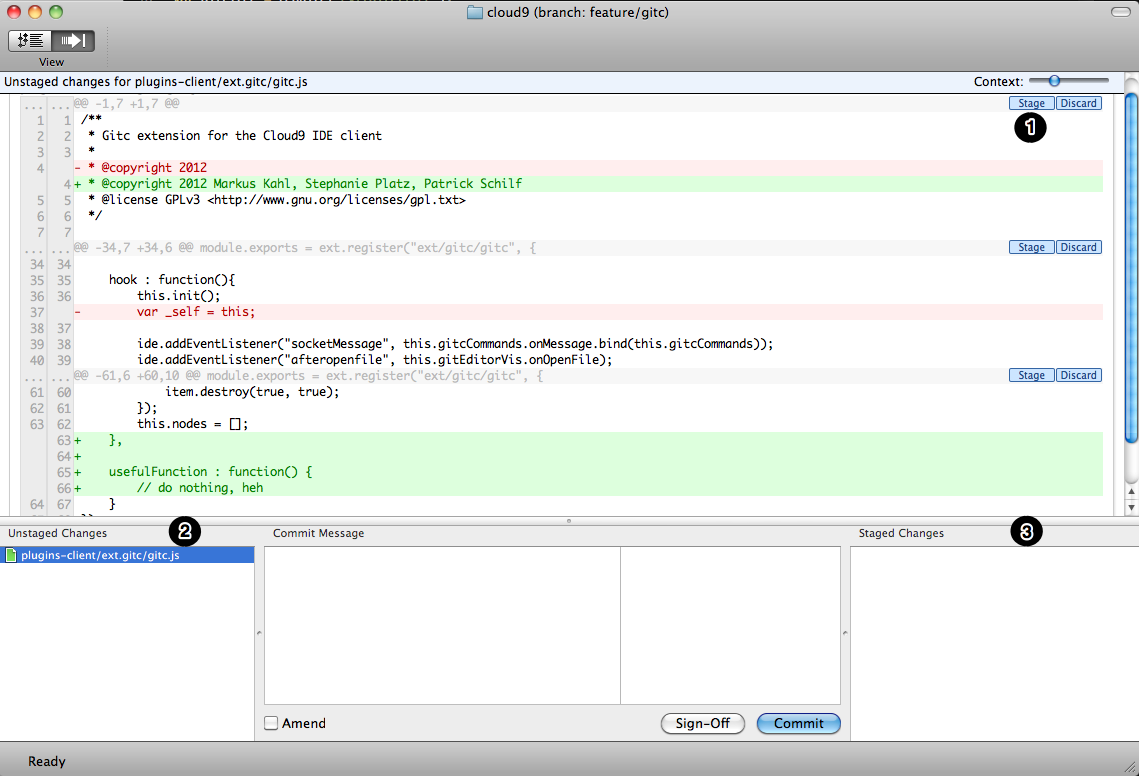
\includegraphics[width=0.9\textwidth]{images/gitx-commit.png}
	\caption{gitx commit view}
	\label{fig:gitx-commit}
\end{figure}

You can see gitx's commit view in figure ~\ref{fig:gitx-commit}. It shows the diff for local changes grouped into several so called hunks by git.
It's also possible to commit those separately by using the command line (\emph{git add --patch}), though gitx offers a more
convenient UI.
As you can see at \circnum{1} there are stage and discard buttons at every hunk.
Through this you can either add separate hunks to the next commit or revert them.
Staged changes will go from \circnum{2} to \circnum{3} and can be unstaged again separately as well.